\documentclass[letterpaper,12pt]{article}

\usepackage{graphicx}
\usepackage{setspace}
\usepackage{enumitem}
\usepackage{natbib}
\usepackage{csquotes}

\begin{document}
\begin{singlespacing}
%\setlist[enumerate]{itemsep=0mm}
%\maketitle

% single or double spacing
%\doublespacing
% \begin{enumerate}
%     \item Identify all the physical and virtual assets in an organization.
%     \item Assign a risk profile to each asset.
%     \item Perform risk evaluation on each asset.
%     \item Perform risk mitigation on each asset.
% \end{enumerate}

% \begin{figure}[h!]
%     \centerline{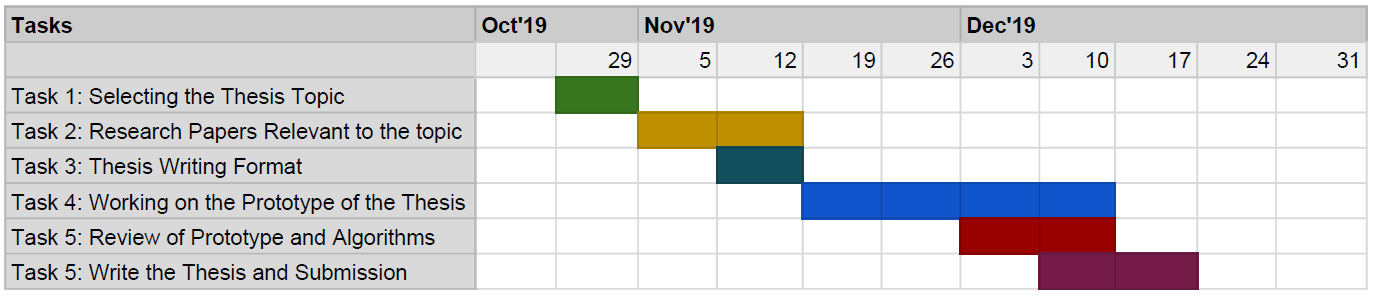
\includegraphics[scale=.45]{GaantChartThesis.PNG}}
%     \caption{Gantt Chart for Litearture Review}
%     %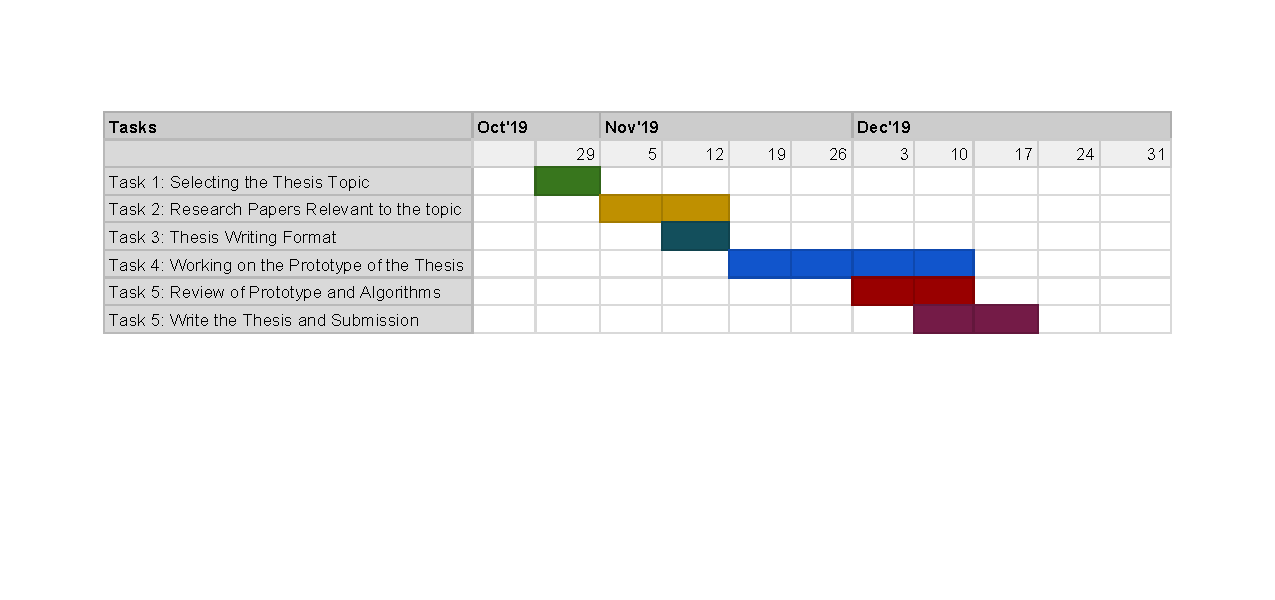
\includegraphics[scale=.8]{GaantChartThesis.pdf}
% \end{figure}

\section*{Purpose}
%This memo is for what ??
The purpose of this document is to summarize the content of my oral presentation and to analyze and evaluate my presentation techniques. The intended audiences of this presentation were my fellow classmates and my ENGR-200W professor, with varying degrees of technical knowledge.

%%%%%%%%%%%%%%%%%%%%%%%%%%%%%%%
%PARTHA'S section starts here
%%%%%%%%%%%%%%%%%%%%%%%%%%%%%%%

\section*{Summary of My Presentation}
%%%%%%%%%%%%%%%%%%%%%%%%%%%%%%%
%PARTHA'S section starts here
%%%%%%%%%%%%%%%%%%%%%%%%%%%%%%%
The presentation starts with an introduction of myself, my interests, and my career goals. In the next slide (slide 4), I place the problem statement, which is the lack of visibility of cyber assets in an enterprise. The cyber assets are not always accounted for in the Information Technology (IT) infrastructure. I propose a solution to this problem by identifying, classifying, ranking, and then managing cyber risks for these assets (slides 5-7). This leads to the introduction of my thesis subject \textquote{Cyber Asset Vulnerability Ranking Algorithm for Security Risk Management} (slide 8). I conclude by explaining how this thesis subject aligns with my career goals (slide 9) and laying out the next steps for this thesis (slide 10).

\section*{Analysis of My Presentation}
\subsection*{Content}
The presentation is intentionally kept short so as to retain the audience's attention. I used \textquote{problem-method-solution} as described in \citep{markel_selber_2018} to explain the topic of my thesis. I used visuals extensively to explain the technical concepts so that they are easily digestible to a non-technical audience. My slides were not heavily worded, which allowed the audience to listen to me. The title of the thesis is introduced late in the presentation by design so as to give the audience enough time to get familiarized with the complex, heavily-worded concept.
\subsection*{Presentation Skills}
My appearance for the presentation was professional. My voice was clear and I was able to articulate my idea in a well structured format. I connected with my audience by asking them questions, thereby engaging them in my presentation. I used effective hand gestures and an engaging body language. For e.g., while talking about the problem statement in slide 5, I was pointing to the projected slides while maintaining eye contact with the audience. I was able to complete the presentation within the stipulated time without rushing through the content. \\
However, there were some room for improvements in my presentation skills. I made a few grammatical mistakes in the initial part of the presentation. For e.g.,\textquote{\ldots if my ideas, kinds of liked by you \ldots }, etc. I used too many fillers at the beginning of my presentation. It may also have been better if I had given my audience a chance to ask questions.

%\section*{Conclusion}

%\nocite{*}

%%%%%%%%%%%%%%%%%%%%%%%%%%%%%%%
%PARTHA'S section starts here
%%%%%%%%%%%%%%%%%%%%%%%%%%%%%%%
\bibliographystyle{apalike}
\bibliography{oralPreso}
\end{singlespacing}
\end{document}
